%%%%%%%%%%%%%%%%%%%%%%%%%%%%%%%%%%%%%%%%%%%%%%%%%%
%% 第2部 開始
%%%%%%%%%%%%%%%%%%%%%%%%%%%%%%%%%%%%%%%%%%%%%%%%%%
\begin{frame}{~}
\centering \Large
\textbf{-- 根付き全域森遷移問題のデモ --}
\end{frame}
%%%%%%%%%%%%%%%%%%%%%%%%%%%%%%%%%%%%%%%%%%%%%%%%%%
%% 遷移問題の入力 (グラフ)
%%%%%%%%%%%%%%%%%%%%%%%%%%%%%%%%%%%%%%%%%%%%%%%%%%
\begin{frame}{問題:入力グラフ}
  \renewcommand{\thefootnote}{\fnsymbol{footnote}}
  \setcounter{footnote}{1}
\begin{textblock*}{\linewidth}(5pt,40pt)
\begin{itemize}
 \item DNET\footnote{https://github.com/takemaru/dnet}
	   \!の例(\code{data/test.yaml})を使用
\end{itemize} 
\end{textblock*}\vfill
\begin{textblock*}{0.4\linewidth}(223pt,25pt)
 \centering
 \fbox{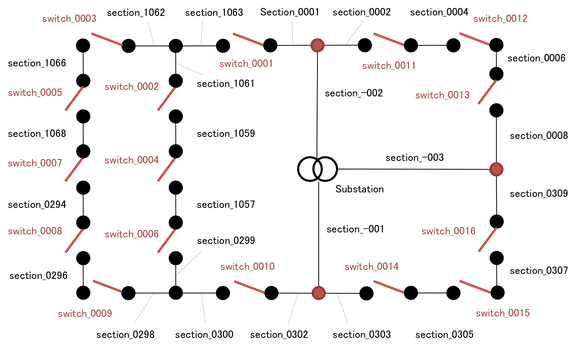
\includegraphics[width=\linewidth]{fig/dnet.png}}
 {\tiny(https://github.com/takemaru/dnetより引用)}
\end{textblock*}\vfill
\scalebox{0.75}{%%%%%%%%%%%%%%%%%%%%%%%%%%%%%%%%%%%%%%%%%%%%%%%%%%
% test.lp
%%%%%%%%%%%%%%%%%%%%%%%%%%%%%%%%%%%%%%%%%%%%%%%%%%

\begin{tikzpicture}

 % 設定
 \tikzset{node/.style={circle,draw=black,fill=white,minimum height=1cm}}

 \definecolor{edgeR}{RGB}{191,0,0}
 \definecolor{nodeR}{RGB}{249,200,200}
 \definecolor{edgeY}{RGB}{255,149,0}
 \definecolor{nodeY}{RGB}{255,231,76}
 \definecolor{edgeB}{RGB}{38,38,134}
 \definecolor{nodeB}{RGB}{200,200,249}

 \tikzset{NodeR/.style={circle,draw=black,fill=nodeR,minimum height=1cm}}
 \tikzset{NodeY/.style={circle,draw=black,fill=nodeY,minimum height=1cm}}
 \tikzset{NodeB/.style={circle,draw=black,fill=nodeB,minimum height=1cm}}

 % 補助線
 % \draw [help lines,blue] (0,0) grid (20,6);

 % 入力されるグラフ
 % node %
 \node[node, ultra thick,draw=edgeR,fill=nodeR] (1) {1};
 \node[node,left= of 1] (2){2};
 \node[node,above= of 2] (3){3};
 \node[node,left= of 2] (4){4};
 \node[node,above= of 3] (5){5};
 \node[node,left= of 3] (6){6};
 \node[node,above= of 5] (7){7};
 \node[node,left= of 5] (8){8};
 \node[node,left= of 7] (9){9};
 \node[node,right= of 7, ultra thick,draw=edgeB,fill=nodeB] (10){10};
 \node[node,right= of 1] (11){11};
 \node[node,right= of 11] (12){12};
 \node[node,above=2cm of 12, ultra thick,draw=edgeY,fill=nodeY] (13){13};
 \node[node,right= of 10] (14){14};
 \node[node,right= of 14] (15){15};

 %\node[rectangle,above=2cm of 1, draw=black,ultra thick,minimum height=1cm] (ss){変電所};

 % 辺
 \foreach \u / \v in {1/2,2/3,2/4,3/5,4/6,5/7,6/8,8/9,7/9,7/10,1/11,11/12,12/13,13/15,14/15,10/14}
 \draw (\u) -- (\v);
\end{tikzpicture}

%%%%%%%%%%%%%%%%%%%%%%%%%%%%%%%%%%%%%%%%%%%%%%%%%%%%%%%%%%
%%% Local Variables:
%%% mode: japanese-latex
%%% TeX-master: ``slide''
%%% End:
}
\begin{textblock*}{0.4\linewidth}(225pt,150pt)
\begin{itemize}
 \item \structure{\bf ノード数: 15}
 \item \structure{\bf 辺数: 16}
 \item \structure{\bf 根ノード数: 3}
\end{itemize}
\end{textblock*}\vfill
\end{frame}
%%%%%%%%%%%%%%%%%%%%%%%%%%%%%%%%%%%%%%%%%%%%%%%%%%
%% 遷移問題の入力 (スタートとゴール)
%%%%%%%%%%%%%%%%%%%%%%%%%%%%%%%%%%%%%%%%%%%%%%%%%%
\begin{frame}{問題:スタート状態とゴール状態}
  \begin{columns}
    \begin{column}{0.45\textwidth}\centering
      \begin{exampleblock}{スタート状態}
	\centering
	\scalebox{0.55}{%%%%%%%%%%%%%%%%%%%%%%%%%%%%%%%%%%%%%%%%%%%%%%%%%%
% test.lp
%%%%%%%%%%%%%%%%%%%%%%%%%%%%%%%%%%%%%%%%%%%%%%%%%%

\begin{tikzpicture}

 % 設定
 \tikzset{node/.style={circle,draw=black,fill=white,minimum height=1cm}}

 \definecolor{edgeR}{RGB}{191,0,0}
 \definecolor{nodeR}{RGB}{249,200,200}
 \definecolor{edgeY}{RGB}{255,149,0}
 \definecolor{nodeY}{RGB}{255,231,76}
 \definecolor{edgeB}{RGB}{38,38,134}
 \definecolor{nodeB}{RGB}{200,200,249}

 \tikzset{NodeR/.style={circle,draw=black,fill=nodeR,minimum height=1cm}}
 \tikzset{NodeY/.style={circle,draw=black,fill=nodeY,minimum height=1cm}}
 \tikzset{NodeB/.style={circle,draw=black,fill=nodeB,minimum height=1cm}}

 % 補助線
 % \draw [help lines,blue] (0,0) grid (20,6);

 % 入力されるグラフ
 % node %
 \node[node, ultra thick,draw=edgeR,fill=nodeR] (1) {1};
 \node[node,left= of 1] (2){2};
 \node[node,above= of 2] (3){3};
 \node[node,left= of 2] (4){4};
 \node[node,above= of 3] (5){5};
 \node[node,left= of 3] (6){6};
 \node[node,above= of 5] (7){7};
 \node[node,left= of 5] (8){8};
 \node[node,left= of 7] (9){9};
 \node[node,right= of 7, ultra thick,draw=edgeB,fill=nodeB] (10){10};
 \node[node,right= of 1] (11){11};
 \node[node,right= of 11] (12){12};
 \node[node,above=2cm of 12, ultra thick,draw=edgeY,fill=nodeY] (13){13};
 \node[node,right= of 10] (14){14};
 \node[node,right= of 14] (15){15};

 %\node[rectangle,above=2cm of 1, draw=black,ultra thick,minimum height=1cm] (ss){変電所};

 % 辺
 % root1
 \foreach \u / \v in {}
 \draw [very thick, edgeR] (\u) -- (\v);
 \foreach \n in {}
 \node[NodeR] at (\n) {\n};
 % root10
 \foreach \u / \v in {10/7,7/9,9/8,8/6,7/5,4/6,2/4,3/2}
 \draw [very thick, edgeB](\u) -- (\v);
 \foreach \n in {7,9,8,6,5,4,3,2}
 \node[NodeB] at (\n) {\n};
 % root13
 \foreach \u / \v in {13/15, 14/15,13/12,11/12}
 \draw [very thick, edgeY] (\u) -- (\v);
 \foreach \n in {15,14,12,11}
 \node[NodeY] at (\n) {\n};

\end{tikzpicture}

%%%%%%%%%%%%%%%%%%%%%%%%%%%%%%%%%%%%%%%%%%%%%%%%%%%%%%%%%%
%%% Local Variables:
%%% mode: japanese-latex
%%% TeX-master: ``slide''
%%% End:
}
      \end{exampleblock}
    \end{column}
    \begin{column}{0.05\textwidth}\centering
      $\Rightarrow$
    \end{column}
    \begin{column}{0.45\textwidth}\centering
      \begin{exampleblock}{ゴール状態}
        \centering
        \scalebox{0.55}{%%%%%%%%%%%%%%%%%%%%%%%%%%%%%%%%%%%%%%%%%%%%%%%%%%
% test.lp
%%%%%%%%%%%%%%%%%%%%%%%%%%%%%%%%%%%%%%%%%%%%%%%%%%

\begin{tikzpicture}

 % 設定
 \tikzset{node/.style={circle,draw=black,fill=white,minimum height=1cm}}

 \definecolor{edgeR}{RGB}{191,0,0}
 \definecolor{nodeR}{RGB}{249,200,200}
 \definecolor{edgeY}{RGB}{255,149,0}
 \definecolor{nodeY}{RGB}{255,231,76}
 \definecolor{edgeB}{RGB}{38,38,134}
 \definecolor{nodeB}{RGB}{200,200,249}

 \tikzset{NodeR/.style={circle,draw=black,fill=nodeR,minimum height=1cm}}
 \tikzset{NodeY/.style={circle,draw=black,fill=nodeY,minimum height=1cm}}
 \tikzset{NodeB/.style={circle,draw=black,fill=nodeB,minimum height=1cm}}

 % 補助線
 % \draw [help lines,blue] (0,0) grid (20,6);

 % 入力されるグラフ
 % node %
 \node[node, ultra thick,draw=edgeR,fill=nodeR] (1) {1};
 \node[node,left= of 1] (2){2};
 \node[node,above= of 2] (3){3};
 \node[node,left= of 2] (4){4};
 \node[node,above= of 3] (5){5};
 \node[node,left= of 3] (6){6};
 \node[node,above= of 5] (7){7};
 \node[node,left= of 5] (8){8};
 \node[node,left= of 7] (9){9};
 \node[node,right= of 7, ultra thick,draw=edgeB,fill=nodeB] (10){10};
 \node[node,right= of 1] (11){11};
 \node[node,right= of 11] (12){12};
 \node[node,above=2cm of 12, ultra thick,draw=edgeY,fill=nodeY] (13){13};
 \node[node,right= of 10] (14){14};
 \node[node,right= of 14] (15){15};

 %\node[rectangle,above=2cm of 1, draw=black,ultra thick,minimum height=1cm] (ss){変電所};

 % 辺
 % root1
 \foreach \u / \v in {1/2,4/6,2/4,3/2,3/5,1/11}
 \draw [very thick, edgeR] (\u) -- (\v);
 \foreach \n in {2,3,4,5,6,11}
 \node[NodeR] at (\n) {\n};
 %root10
 \foreach \u / \v in {10/7,7/9,9/8,10/14,14/15}
 \draw [very thick, edgeB](\u) -- (\v);
 \foreach \n in {7,9,8,14,15}
 \node[NodeB] at (\n) {\n};
 % root13
 \foreach \u / \v in {13/12}
 \draw [very thick, edgeY] (\u) -- (\v);
 \foreach \n in {12}
 \node[NodeY] at (\n) {\n};


\end{tikzpicture}

%%%%%%%%%%%%%%%%%%%%%%%%%%%%%%%%%%%%%%%%%%%%%%%%%%%%%%%%%%
%%% Local Variables:
%%% mode: japanese-latex
%%% TeX-master: ``slide''
%%% End:
}
      \end{exampleblock}
    \end{column}
  \end{columns}\vfill
\begin{itemize}
 \item 問題のASPファクト形式,遷移問題の符号化は\textit{emacs}にて 
\end{itemize}
\end{frame}
%%%%%%%%%%%%%%%%%%%%%%%%%%%%%%%%%%%%%%%%%%%%%%%%%%
%% 遷移問題の実行
%%%%%%%%%%%%%%%%%%%%%%%%%%%%%%%%%%%%%%%%%%%%%%%%%%
\begin{frame}{遷移}
\begin{itemize}
 \only<1>{\item $t=0$ \structure{\bf スタート状態}}
 \only<2>{\item $t=1$}
 \only<3>{\item $t=2$}
 \only<4>{\item $t=3$}
 \only<5>{\item $t=4$ \structure{\bf ゴール状態}}
\end{itemize}\vfill
 \begin{exampleblock}{}
\centering
%%%%%%%%%%%%%%%%%%%%%%%%%%%%%%%%%%%%%%%%%%%%%%%%%%
% test.lp
%%%%%%%%%%%%%%%%%%%%%%%%%%%%%%%%%%%%%%%%%%%%%%%%%%

\begin{tikzpicture}

 % 設定
 \tikzset{node/.style={circle,draw=black,fill=white,minimum height=1cm}}

 \definecolor{edgeR}{RGB}{191,0,0}
 \definecolor{nodeR}{RGB}{249,200,200}
 \definecolor{edgeY}{RGB}{255,149,0}
 \definecolor{nodeY}{RGB}{255,231,76}
 \definecolor{edgeB}{RGB}{38,38,134}
 \definecolor{nodeB}{RGB}{200,200,249}

 \tikzset{NodeR/.style={circle,draw=black,fill=nodeR,minimum height=1cm}}
 \tikzset{NodeY/.style={circle,draw=black,fill=nodeY,minimum height=1cm}}
 \tikzset{NodeB/.style={circle,draw=black,fill=nodeB,minimum height=1cm}}

 % 補助線
 % \draw [help lines,blue] (0,0) grid (20,6);

 % 入力されるグラフ
 % node %
 \node[node, ultra thick,draw=edgeR,fill=nodeR] (1) {1};
 \node[node,left= of 1] (2){2};
 \node[node,above= of 2] (3){3};
 \node[node,left= of 2] (4){4};
 \node[node,above= of 3] (5){5};
 \node[node,left= of 3] (6){6};
 \node[node,above= of 5] (7){7};
 \node[node,left= of 5] (8){8};
 \node[node,left= of 7] (9){9};
 \node[node,right= of 7, ultra thick,draw=edgeB,fill=nodeB] (10){10};
 \node[node,right= of 1] (11){11};
 \node[node,right= of 11] (12){12};
 \node[node,above=2cm of 12, ultra thick,draw=edgeY,fill=nodeY] (13){13};
 \node[node,right= of 10] (14){14};
 \node[node,right= of 14] (15){15};

 %\node[rectangle,above=2cm of 1, draw=black,ultra thick,minimum height=1cm] (ss){変電所};

 \onslide<1>
 % 辺
 % root1
 \foreach \u / \v in {}
 \draw [very thick, edgeR] (\u) -- (\v);
 \foreach \n in {}
 \node[NodeR] at (\n) {\n};
 % root10
 \foreach \u / \v in {10/7,7/9,9/8,8/6,7/5,4/6,2/4,3/2}
 \draw [very thick, edgeB](\u) -- (\v);
 \foreach \n in {7,9,8,6,5,4,3,2}
 \node[NodeB] at (\n) {\n};
 % root13
 \foreach \u / \v in {13/15, 14/15,13/12,11/12}
 \draw [very thick, edgeY] (\u) -- (\v);
 \foreach \n in {15,14,12,11}
 \node[NodeY] at (\n) {\n};

 \onslide<2>
 % 辺
 % root1
 \foreach \u / \v in {1/2,4/6,2/4,3/2}
 \draw [very thick, edgeR] (\u) -- (\v);
 \foreach \n in {2,3,4,6}
 \node[NodeR] at (\n) {\n};
 % root10
 \foreach \u / \v in {10/7,7/9,9/8,7/5}
 \draw [very thick, edgeB](\u) -- (\v);
 \foreach \n in {7,9,8,5}
 \node[NodeB] at (\n) {\n};
 % root13
 \foreach \u / \v in {13/15, 14/15,13/12,11/12}
 \draw [very thick, edgeY] (\u) -- (\v);
 \foreach \n in {15,14,12,11}
 \node[NodeY] at (\n) {\n};

 \onslide<3>
 % 辺
 % root1
 \foreach \u / \v in {1/2,4/6,2/4,3/2}
 \draw [very thick, edgeR] (\u) -- (\v);
 \foreach \n in {2,3,4,6}
 \node[NodeR] at (\n) {\n};
 % root10
 \foreach \u / \v in {10/7,7/9,9/8,7/5,10/14,14/15}
 \draw [very thick, edgeB](\u) -- (\v);
 \foreach \n in {7,9,8,5,14,15}
 \node[NodeB] at (\n) {\n};
 % root13
 \foreach \u / \v in {13/12,11/12}
 \draw [very thick, edgeY] (\u) -- (\v);
 \foreach \n in {12,11}
 \node[NodeY] at (\n) {\n};

 \onslide<4>
 % 辺
 % root1
 \foreach \u / \v in {1/2,4/6,2/4,3/2,3/5}
 \draw [very thick, edgeR] (\u) -- (\v);
 \foreach \n in {2,3,4,5,6}
 \node[NodeR] at (\n) {\n};
 %root10
 \foreach \u / \v in {10/7,7/9,9/8,10/14,14/15}
 \draw [very thick, edgeB](\u) -- (\v);
 \foreach \n in {7,9,8,14,15}
 \node[NodeB] at (\n) {\n};
 % root13
 \foreach \u / \v in {13/12,11/12}
 \draw [very thick, edgeY] (\u) -- (\v);
 \foreach \n in {12,11}
 \node[NodeY] at (\n) {\n};

 \onslide<5>
 % 辺
 % root1
 \foreach \u / \v in {1/2,4/6,2/4,3/2,3/5,1/11}
 \draw [very thick, edgeR] (\u) -- (\v);
 \foreach \n in {2,3,4,5,6,11}
 \node[NodeR] at (\n) {\n};
 %root10
 \foreach \u / \v in {10/7,7/9,9/8,10/14,14/15}
 \draw [very thick, edgeB](\u) -- (\v);
 \foreach \n in {7,9,8,14,15}
 \node[NodeB] at (\n) {\n};
 % root13
 \foreach \u / \v in {13/12}
 \draw [very thick, edgeY] (\u) -- (\v);
 \foreach \n in {12}
 \node[NodeY] at (\n) {\n};

 \onslide<1->

\end{tikzpicture}

%%%%%%%%%%%%%%%%%%%%%%%%%%%%%%%%%%%%%%%%%%%%%%%%%%%%%%%%%%
%%% Local Variables:
%%% mode: japanese-latex
%%% TeX-master: ``slide''
%%% End:

\end{exampleblock}
\end{frame}



